\section{Theorie}
\label{sec:Theorie}
Als Spannungsquelle wird hier ein Gerät verwedet, welches über einen endlichen Zeitraum hinweg eine konstante elektrische Leistung liefert.
Für die Kenntnis über das Verhalten der Spannungsquelle, innerhalb einer elektrischen Schaltung, müssen die Leerlaufspannung und der Innenwiderstand bekannt sein.
Genau dann, wenn der Spannungsquelle kein Strom entnommen wird, dann liegt an ihr die Leerlaufspannung $U_0$ an.
Wenn ein endlicher Strom $\symbf{I}$ durch einen Lastwiderstnd $R_a$ fließt, dann sinkt die Spannung $U_k$, welche an den Ausgangsbuchsen der belasteten Spannungsquelle abgegriffen werden kann, unter $U_0$.
Durch die zuordnung eines Innenwiderstandes $R_i$ zur Spannungsquelle kann dieses Phänomen formal erklärt werden.
Aus der Maschenregl in der Formulierung: "Die Summe aller Spannungsabfälle an den Widerständen $R_m$ der Masche ist gleich die Summe der Leerlaufspnnungen."
\begin{equation}
  \sum\limits{n} U_{0n} = \sum\limits{m} R_m \symbf{I}_m
  \label{eqn:eq1}
\end{equation} 
Nach Abb. \ref{fig:abb1} folgt mit $U_{0_n} = U_0$, $\symbf{I}_m = \symbf{I}$ für $m = 1, 2$, $R_1 = R_i$ und $R_2 = R_a$ die Gleichung
\begin{equation}
  U_0 = \symbf{I} R_i + \symbf{I} R_a
  \label{eqn:eq2}
\end{equation}
\begin{figure}
  \centering
  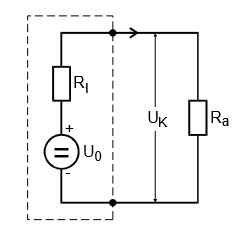
\includegraphics{data/abb1.jpg}
  \caption{Ersatzschaltbild einer realen Spannungsquelle mit Lastwiderstand $R_a$. \cite{V301}}
  \label{fig:abb1}
\end{figure}
Für $U_k$ ergibt sich dann
\begin{equation}
  U_k = \symbf{I} R_a = U_0 - \symbf{I} R_i
  \label{eqn:eq3}
\end{equation}
Daraus folgt das Absinken der Spannung $U_k$ mit zunehmenden Strom.
Durch ein hochohmiges Voltmeter und dem dadurch sehr geringen Strom beim messen der Leerlaufspannung, kann das Glied $\symbf{I} R_i$ in Gleichung \ref{eqn:eq3} vernachlässigt werden.
So gilt $U_k \approx U_0$.
Den Umrandeten Teil in Abb. \ref{fig:abb1} nennt an Ersatzschaltbild einer realen Spannungsquelle.
Durch idealisierte Bauteile, deren Wirkungsweise bekannt ist, wird das elektrische Verhalten eines realen Objekts beschrieben.
Für eine reale Spannungsquelle wird der ohmsche Widerstand $R_i$ und eine dazu in Reihe geschaltete ideale Spannungsquelle benötigt.
Diese ist ideal, weil sie eine von äußeren Einflüssen unabhängige Spannung $U_0$ bei einem Innenwiderstand von null liefert.
Durch $R_i$ kann einer Spannungsquelle auch keine beliebig hohe elektrische Leistung entnommen werden.
Die an $R_a$ abgegebene Leistung $N = \symbf{I}^2 R_a$ durchläuft ein Maximum.
Ist $R_a$ so groß gewählt, dass N maximal wird, wird von Leistungsanpassung gesprochen.
Der Innenwiderstand elektrischer Generatorn ist nicht zwingend durch den Gleichstromwiderstand gegeben, sondern beispielsweise durch einen Rückkopplungsmechanismus.
Somit idt es von Nöten den Innenwiderstand als differentielle Größe einzuführen.
\begin{equation}
  R_i = \frac{dU_k}{d\symbf{I}}
\end{equation}